.
\documentclass{article} % For LaTeX2e
\usepackage{iclr2021_conference,times}

% Optional math commands from https://github.com/goodfeli/dlbook_notation.
\input{math_commands.tex}

\usepackage{hyperref}
\usepackage{url}
\usepackage{tikz}
\usetikzlibrary{positioning,arrows.meta,shapes,calc,fit,matrix}

\title{A trip advisor based on LightRAG}

% Authors must not appear in the submitted version. They should be hidden
% as long as the \iclrfinalcopy macro remains commented out below.
% Non-anonymous submissions will be rejected without review.

\author{Antiquus S.~Hippocampus, Natalia Cerebro \& Amelie P. Amygdale \thanks{ Use footnote for providing further information
about author (webpage, alternative address)---\emph{not} for acknowledging
funding agencies.  Funding acknowledgements go at the end of the paper.} \\
Department of Computer Science\\
Cranberry-Lemon University\\
Pittsburgh, PA 15213, USA \\
\texttt{\{hippo,brain,jen\}@cs.cranberry-lemon.edu} \\
\And
Ji Q. Ren \& Yevgeny LeNet \\
Department of Computational Neuroscience \\
University of the Witwatersrand \\
Joburg, South Africa \\
\texttt{\{robot,net\}@wits.ac.za} \\
\AND
Coauthor \\
Affiliation \\
Address \\
\texttt{email}
}

% The \author macro works with any number of authors. There are two commands
% used to separate the names and addresses of multiple authors: \And and \AND.
%
% Using \And between authors leaves it to \LaTeX{} to determine where to break
% the lines. Using \AND forces a linebreak at that point. So, if \LaTeX{}
% puts 3 of 4 authors names on the first line, and the last on the second
% line, try using \AND instead of \And before the third author name.

\newcommand{\fix}{\marginpar{FIX}}
\newcommand{\new}{\marginpar{NEW}}

%\iclrfinalcopy % Uncomment for camera-ready version, but NOT for submission.
\begin{document}


\maketitle
\vspace{-45pt}
\author[{Fanshi Meng (904055546), Junbo Zou (904145436)}
\section{Introduction}

Recommender systems have become an essential component in the field of information retrieval and decision support, especially in tourism where users expect personalized suggestions for destinations and activities \citep{Ricci2011, Felfernig2018}. Traditional recommendation methods, such as collaborative filtering and content-based approaches, often struggle with capturing complex relationships among entities in a knowledge-rich domain like tourism \citep{Adomavicius2005}.

Recently, Retrieval-Augmented Generation (RAG) has emerged as a promising paradigm that integrates retrieval with large language models, thereby enabling systems to leverage structured or semi-structured knowledge in natural language tasks \citep{Lewis2020}. LightRAG, in particular, extends RAG into the graph domain by introducing graph-structured retrieval mechanisms \citep{Zhu2024}. This allows for modeling of entities and their relationships in a graph, which is highly suitable for domains such as tourism where destinations, attractions, and categories are inherently interconnected.

In this project, we focus on the U.S. state of Georgia as our case study. Georgia offers diverse tourist attractions including natural landscapes, cultural heritage sites, and urban experiences. By representing these attractions and their relationships in a graph structure, we can leverage LightRAG’s graph-based retrieval capabilities to provide more meaningful and context-aware tourism recommendations.

\begin{figure}[htbp]
\centering
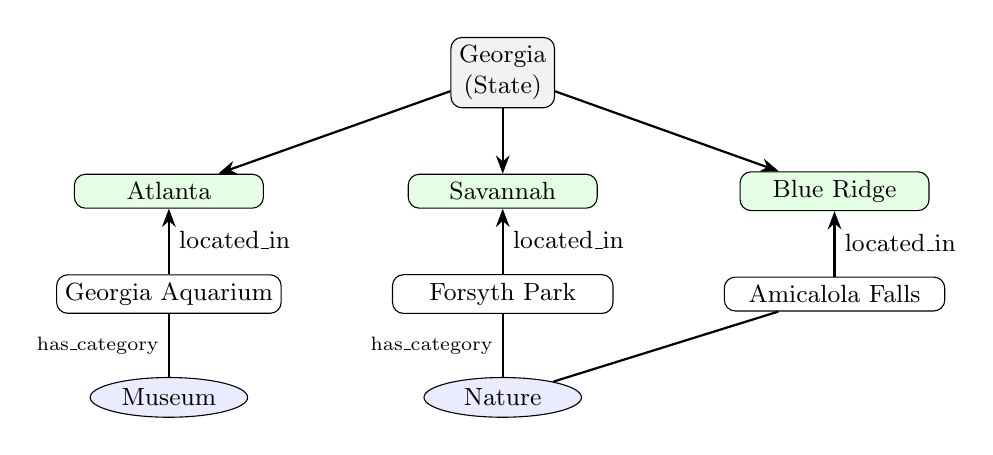
\begin{tikzpicture}[
  >=Stealth,
  font=\small,
  state/.style={draw, rounded corners, fill=gray!10, inner sep=3pt, align=center},
  city/.style={draw, rounded corners, fill=green!10, inner sep=3pt, align=center, minimum width=24mm},
  attr/.style={draw, rounded corners, fill=white, inner sep=3pt, align=center, minimum width=28mm},
  cat/.style={draw, ellipse, fill=blue!8, inner sep=2pt, align=center, minimum width=20mm},
  rel/.style={->, thick},
  catrel/.style={-., thick},
  simrel/.style={<->, densely dotted}
]

% Matrix to keep everything neatly aligned (3 columns)
\matrix[matrix of nodes,
        row sep=8mm,
        column sep=14mm,
        nodes={anchor=center}]
(m){
  % Row 1 (state centered on column 2)
  & \node[state] (ga) {Georgia\\(State)}; & \\
  % Row 2 (cities/regions)
  \node[city] (atl) {Atlanta}; & \node[city] (sav) {Savannah}; & \node[city] (br) {Blue Ridge}; \\
  % Row 3 (one attraction per city)
  \node[attr] (aq) {Georgia Aquarium}; & \node[attr] (fp) {Forsyth Park}; & \node[attr] (af) {Amicalola Falls}; \\
  % Row 4 (categories moved to bottom)
  \node[cat] (museum) {Museum}; & \node[cat] (nature) {Nature}; & \\
};

% State -> Cities/Regions
\draw[rel] (ga) -- (atl);
\draw[rel] (ga) -- (sav);
\draw[rel] (ga) -- (br);

% Attractions -> City/Region
\draw[rel] (aq) -- node[right, pos=0.52]{located\_in} (atl);
\draw[rel] (fp) -- node[right, pos=0.52]{located\_in} (sav);
\draw[rel] (af) -- node[right, pos=0.52]{located\_in} (br);

% Category relations (now to bottom nodes)
\draw[catrel] (aq) -- (museum) node[midway, left] {\scriptsize has\_category};
\draw[catrel] (fp) -- (nature) node[midway, left] {\scriptsize has\_category};
\draw[catrel] (af) -- (nature);

% Optional: example similarity (leave commented if not needed)
% \draw[simrel] (fp) to[bend left=8] node[above]{\scriptsize similar\_to} (af);

\end{tikzpicture}
\caption{LightRAG-oriented tourism graph for Georgia: State $\rightarrow$ City/Region $\rightarrow$ Attraction, with bottom categories linked via \textit{has\_category}; attractions link to their city by \textit{located\_in}.}
\label{fig:ga-tourism-graph-bottom-cats}
\end{figure}
\section{Related Work}

RAG was first introduced as a framework combining neural retrieval with generative models, enabling language models to ground their outputs on external knowledge sources \citep{Lewis2020}. This approach alleviates the problem of parametric knowledge limitations by dynamically retrieving documents during inference. Since its introduction, RAG has become a fundamental paradigm in knowledge-intensive natural language processing.

RAG has been widely applied in domain-specific contexts. In healthcare, RAG-based systems have been developed to assist in clinical decision support and medical question answering, where accuracy and transparency are critical \citep{Lee2023, Jin2023}. In finance, RAG has been leveraged for tasks such as risk assessment, financial report analysis, and market intelligence, enabling domain-expert models to retrieve and reason over structured and unstructured documents \citep{Wang2023}. These implementations demonstrate RAG’s strength in handling knowledge-rich tasks across sensitive domains.

In the context of tourism, RAG is a natural fit given the heterogeneous information sources such as attractions, travel guides, reviews, and geographical knowledge. By constructing structured knowledge graphs or domain corpora, RAG can provide users with more personalized and context-aware recommendations. However, despite its promise, existing RAG systems are not without limitations.

Recent work has highlighted seven major failure modes of RAG, including issues such as retrieval insufficiency, hallucination, and context underutilization \citep{Xu2024}. These findings underscore the importance of addressing fundamental weaknesses in RAG pipelines, particularly when applied to recommendation scenarios where reliability and user trust are essential.

To overcome these shortcomings, LightRAG \citep{Zhu2024} has been proposed as a simplified yet efficient graph-oriented variant of RAG. By integrating graph structures into retrieval, LightRAG is particularly suitable for domains like tourism, where entities and their relationships can be explicitly represented and exploited. Our project builds upon this line of research, focusing on the construction of a Georgia tourism attraction graph and its application to recommendation.


\section{Goal}

The goal of this project is twofold:

\begin{enumerate}
    \item \textbf{Contribution of a graph-structured tourism dataset:} We will construct a graph that represents tourism attractions in Georgia. The graph will encode not only the attractions themselves but also their semantic and geographical relationships, such as "located in," "similar to," or "recommended with."

    \item \textbf{Implementation of a graph-based tourism recommender:} Using LightRAG, we will implement a retrieval-augmented recommendation system that can query this graph structure to suggest attractions to tourists. By combining graph-based retrieval with language model generation, the system aims to deliver context-aware and personalized recommendations, surpassing traditional keyword-based retrieval methods.
\end{enumerate}

\section{Methodology}

\subsection{Knowledge Graph Architecture}

We design a multi-layered knowledge graph to capture user preferences and point-of-interest (POI) characteristics. The graph consists of the following entity types:

\begin{itemize}
    \item \textbf{User:} Represents individual travelers with their historical interactions
    \item \textbf{Interest:} User-expressed interests derived from pinned places
    \item \textbf{Place:} POI entities with attributes (name, type, features, location)
    \item \textbf{Category:} Taxonomic classifications (restaurant, museum, park, etc.)
    \item \textbf{Feature:} POI characteristics (budget-friendly, family-friendly, romantic)
    \item \textbf{Destination:} City or region entities
    \item \textbf{TravelProfile:} Aggregated travel behavior patterns
\end{itemize}

Key relationships include: \texttt{HAS\_INTEREST}, \texttt{PINNED}, \texttt{PREFERS\_CATEGORY}, \texttt{BELONGS\_TO}, \texttt{HAS\_FEATURE}, \texttt{LOCATED\_IN}, and \texttt{HAS\_TRAVEL\_PROFILE}. This graph structure enables multi-hop traversal to discover implicit preferences and contextual associations.

\subsection{LightRAG Integration Pipeline}

The recommendation pipeline integrates LightRAG through four stages, transforming explicit user requests into context-rich queries that leverage historical behavior and implicit preferences.

\begin{enumerate}
    \item \textbf{Context Retrieval:} Upon receiving an itinerary creation request, the system queries the knowledge graph to retrieve multi-faceted user context:
    \begin{itemize}
        \item \textit{Explicit preferences:} User's pinned places and their associated categories, extracted from the Interest module
        \item \textit{Implicit patterns:} Inferred category affinities based on historical itinerary creation (e.g., if 70\% of past trips included museums, assign high weight to cultural attractions)
        \item \textit{Collaborative signals:} Preferences of similar users, identified through graph similarity metrics (e.g., users who pinned overlapping places)
        \item \textit{Behavioral profiles:} Budget constraints, travel mode preferences, and temporal patterns (weekend vs. weekday preferences)
    \end{itemize}

    This retrieval is performed via graph traversal queries (e.g., Cypher in Neo4j) that explore 2-3 hop neighborhoods around the user node, balancing between precision and contextual breadth.

    \item \textbf{Context Enrichment:} The retrieved graph context is synthesized with explicit request parameters to form a unified user preference representation. For instance, if a user requests a \textit{3-day Atlanta trip with \$500 budget}, the system enriches this with:
    \begin{itemize}
        \item Historical data: "User has pinned 5 art museums in past trips"
        \item Inferred preferences: "User avoids nightlife categories"
        \item Collaborative data: "Similar users enjoyed Piedmont Park and Ponce City Market"
    \end{itemize}

    This enrichment layer addresses the \textit{context underutilization} problem in vanilla RAG systems \citep{Xu2024}, ensuring the LLM receives comprehensive background for informed decision-making.

    \item \textbf{Prompt Augmentation:} The language model's system and user messages are dynamically augmented with structured preference context. The enhanced prompt follows this template:

    \begin{verbatim}
System: You are a personalized travel assistant with deep
knowledge of user preferences.

User Context:
- Historical interests: [Art museums (5 pins), Parks (3 pins)]
- Category affinities: {Museum: 0.85, Nature: 0.62, ...}
- Travel style: Budget-conscious, prefers public transit
- Similar travelers enjoyed: [Piedmont Park, High Museum]

User Request:
Generate recommendations for a 3-day Atlanta trip with
$500 budget using public transit.
    \end{verbatim}

    This context injection enables the LLM to ground its recommendations in personalized evidence rather than generic popularity, addressing the hallucination problem in RAG \citep{Xu2024}.

    \item \textbf{Graph Update:} After generating recommendations, the system performs incremental knowledge graph updates to capture new preference signals:
    \begin{itemize}
        \item Create edges: \texttt{User -[CREATED\_ITINERARY]-> Itinerary}
        \item Update weights: Strengthen \texttt{PREFERS\_CATEGORY} edges based on selected places
        \item Infer new features: If user selects multiple "outdoor" places, create or strengthen \texttt{User -[LIKES\_FEATURE]-> Feature(outdoor)}
    \end{itemize}

    These updates employ a time-decay mechanism to prioritize recent preferences, enabling the system to adapt to evolving user interests over time.
\end{enumerate}

\subsection{Dual-Level Retrieval Strategy}

A key innovation of LightRAG is its dual-level retrieval mechanism, which combines direct entity matching with relationship-based exploration to capture both explicit and implicit preference signals \citep{Zhu2024}. This addresses a fundamental limitation of traditional RAG systems: the inability to reason about \textit{connections between} entities, not just the entities themselves.

\subsubsection{Entity-Level Retrieval}

Entity-level retrieval performs direct node matching based on semantic similarity between the user query and graph entities. For example:

\begin{itemize}
    \item \textbf{Query:} "I want to visit museums in Atlanta"
    \item \textbf{Retrieval:} Directly fetch \texttt{Place} nodes where:
    \begin{itemize}
        \item \texttt{Place.category = "museum"}
        \item \texttt{Place.location = "Atlanta"}
        \item \texttt{Place.embedding} has high cosine similarity to query embedding
    \end{itemize}
    \item \textbf{Result:} \{High Museum of Art, Fernbank Museum, Atlanta History Center\}
\end{itemize}

This level operates analogously to traditional vector search in RAG, retrieving entities whose attributes or embeddings closely match the query. However, it captures only \textit{first-order} information—entities that directly satisfy the query constraints.

\subsubsection{Relationship-Level Retrieval}

Relationship-level retrieval explores the \textit{graph topology} around retrieved entities, discovering implicit associations through multi-hop traversal. Continuing the above example:

\begin{itemize}
    \item \textbf{Starting from:} High Museum of Art (retrieved via entity-level)
    \item \textbf{Graph traversal:}
    \begin{enumerate}
        \item Follow \texttt{SIMILAR\_TO} edges: Discover "Michael C. Carlos Museum" (similar cultural institution)
        \item Follow \texttt{RECOMMENDED\_WITH} edges: Discover "Piedmont Park" (often visited together)
        \item Follow \texttt{User -[PINNED]-> Place} paths: Find users who pinned High Museum, then retrieve \textit{their} other pinned places (collaborative filtering)
    \end{enumerate}
    \item \textbf{Result:} \{Carlos Museum, Piedmont Park, Ponce City Market\} (not directly matching "museum" but contextually relevant)
\end{itemize}

This captures \textit{second-order and third-order} information—entities that are \textit{related to} the query through the graph structure, enabling serendipitous discovery.

\subsubsection{Why Both Levels Are Necessary}

The two levels serve complementary purposes:

\begin{enumerate}
    \item \textbf{Precision vs. Diversity Tradeoff:}
    \begin{itemize}
        \item Entity-level ensures \textit{relevance}: Retrieved nodes directly match query constraints
        \item Relationship-level ensures \textit{diversity}: Related nodes introduce variety and avoid filter bubbles
    \end{itemize}

    \item \textbf{Cold Start Problem:}
    \begin{itemize}
        \item For new users with no historical data, entity-level retrieval alone would yield generic popular attractions
        \item Relationship-level retrieval enables \texttt{User -[SIMILAR\_TO]-> User} traversal to borrow preferences from similar users based on demographics or initial survey responses
    \end{itemize}

    \item \textbf{Query Ambiguity Handling:}
    \begin{itemize}
        \item Vague queries like "fun things to do in Atlanta" may match many entity types weakly
        \item Relationship-level retrieval resolves ambiguity by considering \textit{co-occurrence patterns}: if parks and restaurants are frequently visited together, both are retrieved
    \end{itemize}

    \item \textbf{Explainability:}
    \begin{itemize}
        \item Entity-level provides transparent rationale: "Recommended because you like museums"
        \item Relationship-level provides discovery rationale: "Users who visited X also enjoyed Y"
    \end{itemize}
\end{enumerate}

\subsubsection{Fusion Strategy}

Retrieved results from both levels are fused using a weighted scoring function:

\begin{equation}
\text{score}(p) = \alpha \cdot \text{sim}_{\text{entity}}(p, q) + \beta \cdot \text{sim}_{\text{path}}(p, q) + \gamma \cdot \text{popularity}(p)
\end{equation}

where:
\begin{itemize}
    \item $\text{sim}_{\text{entity}}(p, q)$: Cosine similarity between place $p$ and query $q$ embeddings
    \item $\text{sim}_{\text{path}}(p, q)$: Path-based score (e.g., inverse shortest path length from user-pinned places to $p$)
    \item $\text{popularity}(p)$: Global popularity score (e.g., PageRank on the place graph)
    \item $\alpha, \beta, \gamma$: Learned weights balancing precision, diversity, and popularity
\end{itemize}

This fusion enables the system to balance between satisfying explicit user intent (entity-level) and providing delightful discovery (relationship-level), a capability absent in conventional RAG systems that operate solely on document-level retrieval.


\bibliography{iclr2021_conference}
\bibliographystyle{iclr2021_conference}


\end{document}
